\documentclass[10pt]{standalone}
\usepackage{amsmath}
\usepackage{pgf,tikz}\usepackage{pgfplots}

\usepackage{mathrsfs}
\usetikzlibrary{arrows}
\pagestyle{empty}
\begin{document}
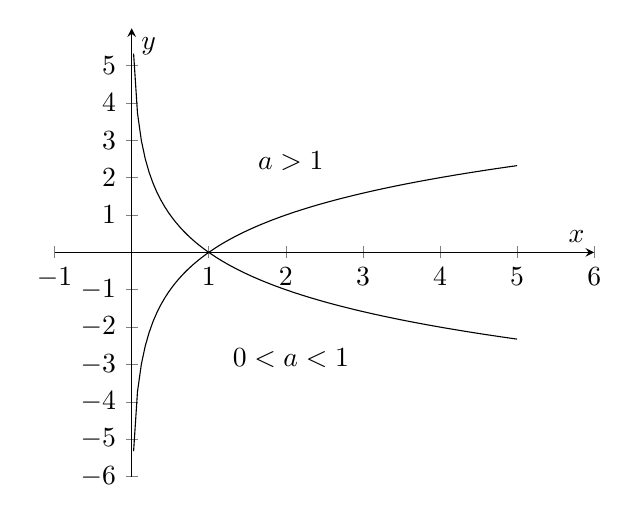
\begin{tikzpicture}
\begin{axis}
[xmin=-1,xmax=6,ymin=-6,ymax=6, %grid,
axis x line=middle,xtick={-1,0,...,6},ytick={-6,-5,...,5},
axis y line=middle,xlabel=$x$,ylabel=$y$]
%\addplot[samples=200] {(1ì^(x))};
%\addplot [samples=200] {(0.83^(x))};
%\addplot [samples=200] {(0.67^(x))};
%\addplot [samples=200] {(0.5^(x))};
\addplot [samples=200]{ln(x)/ln(2)};
\addplot [samples=200]{ln(x)/ln(0.5)};
\end{axis}
\node (a1) at (3,4) {$a>1$};
\node (a1) at (3,1.5) {$0<a<1$};
%\node (a2) at (1,2.2) {$y=(\dfrac{5}{6})^x$};
%\node (a3) at (1.1,4.2) {$y=(\dfrac{2}{3})^x$};
%\node (a3) at (2.1,5) {$y=\dfrac{1}{2}^x$};
\end{tikzpicture}
\end{document}